\documentclass[11pt,letter, swedish, english
]{article}
\pdfoutput=1

\usepackage{../custom_as}
\usepackage[makeroom
]{cancel}
\usepackage{esint}
\let\oldint\int 
\renewcommand{\int}{\oldint\limits}
\graphicspath{{figures/}}

\swapcommands{\Phi}{\varPhi}
\swapcommands{\Omega}{\varOmega}

\newcommand{\enaught}{\ensuremath\varepsilon_0}

%%Drar in tabell och figurtexter
\usepackage[margin=10 pt]{caption}
%%För att lägga in 'att göra'-noteringar i texten
\usepackage{todonotes} %\todo{...}

%%För att själv bestämma marginalerna. 
\usepackage[
%            top    = 2.5cm,
%            bottom = 3cm,
%            left   = 3cm, right  = 3cm
]{geometry}

%%För att ändra hur rubrikerna ska formateras


%\renewcommand{\thefootnote}{\fnsymbol{footnote}}

%\newcommand{\Tc}{\ensuremath{T_{\text{c}}}}
\newcommand{\sign}{\ensuremath{\,\text{sign}}}

%\usepackage{tikz}


\renewcommand{\thesubsection}{\arabic{section} (\alph{subsection})}
\renewcommand{\thesubsubsection}{\arabic{section} (\alph{subsection},\,\roman{subsubsection})}


\begin{document}

%\tikzstyle{every picture}+=[remember picture]
%\tikzstyle{na} = [shape=rectangle,inner sep=0pt,text depth=0pt]



%%%%%%%%%%%%%%%%% vvv Inbyggd titelsida vvv %%%%%%%%%%%%%%%%%

\title{E\&M -- PHYS\,706 \\
Assignment 1}
\author{Andréas Sundström}
\date{\today}

\maketitle

%%%%%%%%%%%%%%%%% ^^^ Inbyggd titelsida ^^^ %%%%%%%%%%%%%%%%%

\section{Electric potential and filed along the $z$ axis}
\begin{figure}\centering
\input{figures/1_geometry.pdf_t}
\caption{The geometry of this problem. Two point charges, each of
  charge $+Q$, are located at $z=\pm R$, and a circular ring centered
  atround the origin with a total charge of $-2Q$.}
\label{fig:1_geometry}
\end{figure}

In this problem, we are tasked to find the electric field and
potential along the $z$~axis, from a geometry given in
\figref{fig:1_geometry}. 

\subsection{The electro static potential}
By the superposition principles we can easili solve this problem in
parts by combining the potentials from each source
$\Phi=\Phi_{+R}+\Phi_{-R}+\Phi_{\text{ring}}$. 

Let's begin with the teo easiest terms. The two terms from the point
charges, which we all know is just
\begin{equation}\label{eq:1_Phi_dot}
\Phi_{\pm{R}}(\vb*r=z\vu{z})=\frac{Q}{4\pi\enaught}
\frac{1}{\abs{\vb*r\mp R\vu{z}}}
=\frac{Q}{4\pi\enaught} \frac{1}{\abs{z\mp R}}.
\end{equation}

Next up is the ring charge. In this case we could easily argue that
the symmetry of the circular charge will make the potential due to
that ring 
\begin{equation}\label{eq:1_Phi_ring}
\Phi_\text{ring}(\vb*r=z\vu{z})=\frac{-2Q}{4\pi\enaught}
\frac{1}{\sqrt{z^2+R^2}},
\end{equation}
where $\sqrt{z^2+R^2}$ is the distance from any point of the ring to
the $z$~axis at $z$. But let's do it more rigorously this time. In
cylindrical coordinates the charge distribution of that ring is
\begin{equation}
\rho(r, \phi, z)=\lambda \delta(z)\delta(r-R),
\end{equation}
where $\lambda=-2Q/(2\pi R)$ is the uniform linear charge density
along the ring. 
Therefore the potential, at any point in space, due to that ring is
\begin{equation}
\Phi_\text{ring}(y, x, z)=\frac{\lambda}{4\pi\enaught}
\int_0^{2\pi}\rd\phi'\int_{-\infty}^\infty\rd{z'}\int_0^\infty\rd{r'}\,r'
\frac{\delta(z)\delta(r-R)}{\abs{\vb*r-\vb*r'}}
\end{equation}
which upon evaluating the $\delta$ functions yields
\begin{equation}
\Phi_\text{ring}(y, x, z)
= \frac{\lambda}{4\pi\enaught} \int_0^{2\pi}\rd\phi'
\frac{R}{\sqrt{(x-R\cos\phi')^2+(y-R\sin\phi'^2)+z^2}}.
\end{equation}
From here, we can clearly see that by setting $x=y=0$ the expression
in the denominator simplifies to $\sqrt{z^2+R^2}$, which is
independent of $\phi'$; we thus end up with exactly
\eqref{eq:1_Phi_ring} as the potential due to the ring on the
$z$~axis.  

The end result from all three sources therefore becomes
\begin{align}\label{eq:1_Phi_a}
\Phi(\vb*r=z\vu{z})=&\frac{Q}{4\pi\enaught}
\qty[\frac{1}{\abs{z-R}}+\frac{1}{\abs{z+R}}
-\frac{2}{\sqrt{z^2+R^2}}]
\\\label{eq:1_Phi_b}
=&\frac{Q}{4\pi\enaught z}
\qty[\frac{1}{\abs{1-R/z}}+\frac{1}{\abs{1+R/z}}
-\frac{2}{\sqrt{1+(R/z)^2}}].
\end{align}

\subsection{The electric field along the $z$ axis}
To calculate the $E$~field along the $z$~axis we use
$\vb*E=-\grad\Phi$, meaning that $E_z=-\pdv*{\Phi}{z}$. This
derivative is easiest done using \eqref{eq:1_Phi_a}. We begin by
rewriting the absolute values\footnotemark, then we differentiate:
\begin{equation}
\begin{aligned}
E_z(\vb*r=z\vu{z})=&
-\frac{Q}{4\pi\enaught} \pdv{z}\qty[
\frac{\sign(z-R)}{(z-R)} +\frac{\sign(z+R)}{(z+R)}
-\frac{2}{\sqrt{z^2+R^2}}]\\
=&-\frac{Q}{4\pi\enaught} \qty[
-\frac{\sign(z-R)}{(z-R)^2} -\frac{\sign(z+R)}{(z+R)^2}
+\frac{2z}{(z^2+R^2)^{3/2}}].
\end{aligned}
\end{equation}
If we want to, we can rewrite this expression as
\begin{equation}
E_z(\vb*r=z\vu{z})
=\frac{Q}{4\pi\enaught z^2} \qty[
\frac{\sign(z-R)}{(1-R/z)^2} +\frac{\sign(z+R)}{(1+R/z)^2}
-\frac{2\sign(z)}{(1+(R/z)^2)^{3/2}}].
\end{equation}
\footnotetext{We are not concerned about the derivatives of the
  ``sign'' functions at their switching point since the rest of the
  expression is not analytic there either. }


\subsection{Asymptotic behaviour of the potential along the $z$ axis}
To find the asymptotic behaviour as $z\to+\infty$, we will need to use
the following Taylor expansion
\begin{equation}
(1+x)^\alpha=1+\alpha x+\frac{\alpha(\alpha-1)}{2}x^2+\order{x^3}
\end{equation}
for sufficiently small $x$. 

In our case, with $\zeta=R/z$, that would correspond to
\begin{equation}
(1\pm\zeta)^{-1}=1\mp\zeta+\zeta^2+\order{\zeta^3}
\end{equation}
and
\begin{equation}
\qty(1+\zeta^2)^{-1/2}=1-\frac{1}{2}\zeta^2+\order{\zeta^4}
\end{equation}
Subsituting these expansions into \eqref{eq:1_Phi_b} gives us the
asymptotic behaviour
\begin{equation}
\Phi(\vb*r=z\vu{z})\sim
\frac{Q}{4\pi\enaught z}
\qty[\qty(1-\zeta+\zeta^2)+\qty(1+\zeta+\zeta^2)
-2\qty(1-\frac{1}{2}\zeta^2)]
=\frac{3Q}{4\pi\enaught}\frac{R^2}{z^3},
\end{equation}
as $\zeta\to0$ or $z\to\infty$.




\section{Charged balls}
\renewcommand{\thesubsection}{\arabic{section} (\roman{subsection})}
This problem concerns charged balls, of radius a, with different chrge
distribution but all with a total charge $Q$. We will be calculating
the $E$-field produced by these charge distributions. 

One generla remark about these fields is that the all have to be of
the form $\vb*E=E_r\vu{r}$, where $\vu{r}$ is the radial unit vector
of a spherical coordinate system. This is due to the spherical
symmetry in this problem. 


\figref{fig:2_e-field} shows a plot of the non-dimensionalized field
strengths as a function of the non-dimensionlized radius
$\xi=r/a$. This is the result of the calculations below. Note that
only the conducting ball produces a discontinuous filed.

\begin{figure}\centering
% GNUPLOT: LaTeX picture with Postscript
\begingroup
  \makeatletter
  \providecommand\color[2][]{%
    \GenericError{(gnuplot) \space\space\space\@spaces}{%
      Package color not loaded in conjunction with
      terminal option `colourtext'%
    }{See the gnuplot documentation for explanation.%
    }{Either use 'blacktext' in gnuplot or load the package
      color.sty in LaTeX.}%
    \renewcommand\color[2][]{}%
  }%
  \providecommand\includegraphics[2][]{%
    \GenericError{(gnuplot) \space\space\space\@spaces}{%
      Package graphicx or graphics not loaded%
    }{See the gnuplot documentation for explanation.%
    }{The gnuplot epslatex terminal needs graphicx.sty or graphics.sty.}%
    \renewcommand\includegraphics[2][]{}%
  }%
  \providecommand\rotatebox[2]{#2}%
  \@ifundefined{ifGPcolor}{%
    \newif\ifGPcolor
    \GPcolortrue
  }{}%
  \@ifundefined{ifGPblacktext}{%
    \newif\ifGPblacktext
    \GPblacktexttrue
  }{}%
  % define a \g@addto@macro without @ in the name:
  \let\gplgaddtomacro\g@addto@macro
  % define empty templates for all commands taking text:
  \gdef\gplbacktext{}%
  \gdef\gplfronttext{}%
  \makeatother
  \ifGPblacktext
    % no textcolor at all
    \def\colorrgb#1{}%
    \def\colorgray#1{}%
  \else
    % gray or color?
    \ifGPcolor
      \def\colorrgb#1{\color[rgb]{#1}}%
      \def\colorgray#1{\color[gray]{#1}}%
      \expandafter\def\csname LTw\endcsname{\color{white}}%
      \expandafter\def\csname LTb\endcsname{\color{black}}%
      \expandafter\def\csname LTa\endcsname{\color{black}}%
      \expandafter\def\csname LT0\endcsname{\color[rgb]{1,0,0}}%
      \expandafter\def\csname LT1\endcsname{\color[rgb]{0,1,0}}%
      \expandafter\def\csname LT2\endcsname{\color[rgb]{0,0,1}}%
      \expandafter\def\csname LT3\endcsname{\color[rgb]{1,0,1}}%
      \expandafter\def\csname LT4\endcsname{\color[rgb]{0,1,1}}%
      \expandafter\def\csname LT5\endcsname{\color[rgb]{1,1,0}}%
      \expandafter\def\csname LT6\endcsname{\color[rgb]{0,0,0}}%
      \expandafter\def\csname LT7\endcsname{\color[rgb]{1,0.3,0}}%
      \expandafter\def\csname LT8\endcsname{\color[rgb]{0.5,0.5,0.5}}%
    \else
      % gray
      \def\colorrgb#1{\color{black}}%
      \def\colorgray#1{\color[gray]{#1}}%
      \expandafter\def\csname LTw\endcsname{\color{white}}%
      \expandafter\def\csname LTb\endcsname{\color{black}}%
      \expandafter\def\csname LTa\endcsname{\color{black}}%
      \expandafter\def\csname LT0\endcsname{\color{black}}%
      \expandafter\def\csname LT1\endcsname{\color{black}}%
      \expandafter\def\csname LT2\endcsname{\color{black}}%
      \expandafter\def\csname LT3\endcsname{\color{black}}%
      \expandafter\def\csname LT4\endcsname{\color{black}}%
      \expandafter\def\csname LT5\endcsname{\color{black}}%
      \expandafter\def\csname LT6\endcsname{\color{black}}%
      \expandafter\def\csname LT7\endcsname{\color{black}}%
      \expandafter\def\csname LT8\endcsname{\color{black}}%
    \fi
  \fi
  \setlength{\unitlength}{0.0500bp}%
  \begin{picture}(7936.00,3968.00)%
    \gplgaddtomacro\gplbacktext{%
      \csname LTb\endcsname%
      \put(860,640){\makebox(0,0)[r]{\strut{} 0}}%
      \put(860,1412){\makebox(0,0)[r]{\strut{} 0.5}}%
      \put(860,2184){\makebox(0,0)[r]{\strut{} 1}}%
      \put(860,2955){\makebox(0,0)[r]{\strut{} 1.5}}%
      \put(860,3727){\makebox(0,0)[r]{\strut{} 2}}%
      \put(980,440){\makebox(0,0){\strut{} 0}}%
      \put(2629,440){\makebox(0,0){\strut{} 0.5}}%
      \put(4278,440){\makebox(0,0){\strut{} 1}}%
      \put(5926,440){\makebox(0,0){\strut{} 1.5}}%
      \put(7575,440){\makebox(0,0){\strut{} 2}}%
      \put(160,2183){\rotatebox{-270}{\makebox(0,0){\strut{}$e(\xi)=E_r(r)\frac{4\pi\enaught a^2}{Q}$}}}%
      \put(4277,140){\makebox(0,0){\strut{}$\xi=(r/a)$}}%
    }%
    \gplgaddtomacro\gplfronttext{%
      \csname LTb\endcsname%
      \put(6792,3514){\makebox(0,0)[r]{\strut{}Conducting ball ($n\to\infty$)}}%
      \csname LTb\endcsname%
      \put(6792,3314){\makebox(0,0)[r]{\strut{}$n=0$}}%
      \csname LTb\endcsname%
      \put(6792,3114){\makebox(0,0)[r]{\strut{}$n=-2$}}%
      \csname LTb\endcsname%
      \put(6792,2914){\makebox(0,0)[r]{\strut{}$n=2$}}%
    }%
    \gplbacktext
    \put(0,0){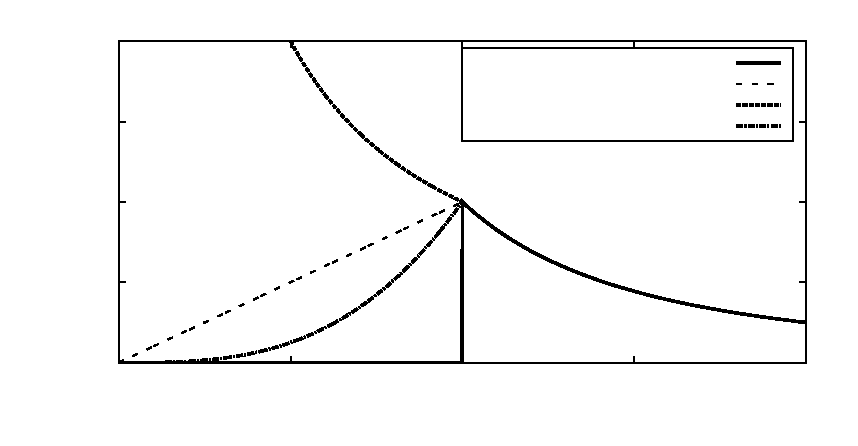
\includegraphics{2_e-field}}%
    \gplfronttext
  \end{picture}%
\endgroup

\caption{A non-dimensionalized plot of some of the electric filed
  strengths produced by the charged balls of radius $\xi=r/a=1$. The first
  graph is the field from a conducting ball, and the three others are
  from balls with charge densities $\rho\propto\xi^n$.}
\label{fig:2_e-field}
\end{figure}

\subsection{Conductive ball}
In this care, we are not explicitly given any chrge distribution, but
we should know by now that all charge on a conductor will gather on
the surface. In other words, there will be no $E$~filed inside the
bulk of the conductor. To show this we can, for instance, use the fact
that $\Phi$ is constant in a conductor; then we 
clearly see that $\vb*E=-\grad\Phi=\vb0$. Furthermore since we have a
ball, the spherical symmetry will result in the charge being evenly
distributed over the surface. 

Now to the field produced by this ball. By applying Gauss's law on
a spherical Gauss surface $S_R$, of radius $R>a$, we get
\begin{equation}
\oiint\limits_{S_R}E_r\vu{r}\vdot\rd\vb*{A}
=\frac{1}{\enaught}\iiint\limits_{V_R} \rho(\vb*r)\id{V}
=\frac{Q}{\enaught}.
\end{equation}
Now since $E_r$ is constant on $S_R$ and $\rd\vb*A=\vu{r}\rd{A}$, the
LHS is just $4\pi R^2\, E_r\!(R)$. The full expression for the $E$~field is
now
\begin{equation}
E_r(r)=
\begin{cases}
0, &r<a,\\
\frac{Q}{4\pi\enaught r^2}\qcomma &r>a,
\end{cases}
\end{equation}
and $\vb*E=E_r\vu{r}$.

We can also note that the field outside any of the balls in this
problem will be the same. This is due to the fact that enclosed charge
by any surface enclosing the whole ball will be~$Q$. 

\subsection{Uniform charge density}
This time we have to use Gauss's law inside the surface as
well. However, the RHS still has the same form. The charge density
will of course be $\rho(r<a)=Q/(4\pi a^3/3)$.
We therefore get
\begin{equation}
4\pi R^2 E_r(R<a)
=\frac{1}{\enaught}\iiint\limits_{V_R}
\frac{3Q}{4\pi a^3}\id{V}
=\frac{Q}{\enaught}\frac{R^3}{a^3}.
\end{equation}
And the final result is
\begin{equation}
E_r(r)=\frac{Q}{4\pi\enaught}\times
\begin{cases}
\frac{r}{a^3}, &r<a,\\
\frac{1}{r^2}\qcomma &r>a.
\end{cases}
\end{equation}

\subsection{Power relation}
In this case we have a power relation for the charge density
$\rho(r<a)\propto r^n$, $n>-3$; i.e. $\rho(r<a)=(r/a)^n\rho_0$. We
have to begin with calculating $\rho_0$. To do this we note that
\begin{equation}\label{eq:2_rho_0}
Q=\iiint\limits_{V_{a}}\rho(r)\id{V}
=\frac{\rho_0}{a^n}\int_0^{2\pi}\rd\phi\int_0^\pi\sin\theta\id\theta
\int_0^a r^n\,r^2\rd{r}
=\frac{4\pi \rho_0}{a^n}\,\frac{a^{n+3}}{n+3}
\end{equation}
so
\begin{equation}
\rho_0=\frac{(n+3)Q}{4\pi a^3}.
\end{equation}

Now to the electric field. We once again use Gauss's law, which will
just be the same integral as in \eqref{eq:2_rho_0} but with 
$a\to R$. So we get
\begin{equation}
4\pi R^2  E_r(R<a)
=\frac{\rho_0}{a^n\enaught}\iiint\limits_{V_R}r^n\id{V}
=\frac{4\pi\rho_0}{a^n\enaught}\,\frac{R^{n+3}}{n+3}
=\frac{Q}{\enaught}\qty(\frac{R}{a})^{n+3},
\end{equation}
and the final electric field will be
\begin{equation}
E_r(r)=\frac{Q}{4\pi\enaught a^2}\times
\begin{cases}
\qty(\frac{r}{a})^{n+1}, &r<a,\\
\qty(\frac{r}{a})^{-2}\qcomma &r>a.
\end{cases}
\end{equation}

Also note that the previous cases just were special cases of this
case. It's easy to see this for the uniform charge distribution, where
$n=0$. But we can reproduce the same behaviour (pointwise) for the
conducting shpere by letting $n\to\infty$.



\section{Mean charge distribution of a hydrogen atom}
\renewcommand{\thesubsection}{\arabic{section} (\alph{subsection})}
Given the mean potential 
\begin{equation}
\Phi(r)=\frac{q}{4\pi\enaught}\,\frac{\ee^{-\alpha r}}{r}
\qty(1+\frac{\alpha r}{2})
\end{equation}
of a neutral hydrogen atom, we now want to find the charge
distribution $\rho(r)$ that would give rise to such a potential.

We begin with the Poisson equation
\begin{equation}
-\laplacian\Phi=\frac{\rho(r)}{\enaught}.
\end{equation}
Then we need to express the Laplacian in spherical coordinates
\begin{equation}
\laplacian f = \frac{1}{r}\pdv[2]{r}[rf] + 
\text{``Derivatives in }\phi\text{ and }\theta\text{''}.
\end{equation}
We only need the $r$ derivatives since we see that $\Phi$ is
spherically symmetric. 

Finding $\rho$ now is just a matter of doing the derivatives
\begin{equation}
\frac{1}{r}\pdv[2]{r}\qty[\ee^{-\alpha r}
\qty(1+\frac{\alpha r}{2})]
=\frac{1}{r} \qty[-\alpha^2\ee^{-\alpha r} 
+\alpha^2\ee^{-\alpha r}\qty(1+\frac{\alpha r}{2})]
=\frac{\alpha^3}{2}\ee^{-\alpha r} 
\end{equation}
So the charge distribution resulting from
this is
\begin{equation}
\rho'(r)=-q\frac{\alpha^3}{8\pi}\ee^{-\alpha r}.
\end{equation}
This would correspond to $-q$ times the electron's probability density
around the nucleus for a ``1s'' state. It is also easy to see that 
\begin{equation}\label{eq:3_q'}
\iiint \rho'(r)\id{V}=-q,
\end{equation}
which means that we have one ``whole'' electron here.

There is one problem thogh; the potential was that of a \emph{neutral}
hydrogen atom. And we can also see that\footnotemark{}
\begin{equation}\label{eq:3_Phi'}
\begin{aligned}
\Phi'(R)&=\frac{1}{4\pi\enaught}\int_0^{2\pi}\rd\phi\int_0^\pi\sin\theta\id\theta
\int_0^\infty\rd{r}\, 
r^2\frac{\rho'(r)}{\sqrt{R^2+r^2-2Rr\cos\theta}}\\
&=\frac{1}{2\enaught}\int_0^\infty\rd{r}\,
\qty(-\frac{q\alpha^3}{8\pi})r^2\ee^{-\alpha r}
\int_0^\pi\frac{\sin\theta\,\rd\theta}{\sqrt{R^2+r^2-2Rr\cos\theta}}\\
\end{aligned}
\end{equation}
To do the $\theta$ integral, we can substitute $u=\cos\theta$ giving
$\rd{u}=-\sin\theta\id\theta$. The $\theta$ integral therefore becomes
\begin{equation}
\begin{aligned}
\int_0^\pi\frac{\sin\theta\,\rd\theta}{\sqrt{R^2+r^2-2Rr\cos\theta}}
=&\int_{-1}^1\frac{\rd{u}}{\sqrt{R^2+r^2-2Rru}}\\
=&-\frac{1}{Rr}\eval{\sqrt{R^2+r^2-2Rru}}_{-1}^1\\
=&\frac{1}{Rr}\Big(|R+r|-|R-r|\Big)
&=\begin{cases}
2/R\qcomma&R>r\\
2/r,&-r<R<r\\
-2/R,&R<-r.
\end{cases}
\end{aligned}
\end{equation}
When we plug this back into \eqref{eq:3_Phi'}, we get
\begin{equation}\label{eq:3_Phi'_final}
\begin{aligned}
\Phi'(R)=&-\frac{q\alpha^3}{16\pi\enaught}\qty{
\int_0^R\frac{2}{R}r^2\ee^{-\alpha r}\id{r}
+\int_R^\infty\frac{2}{r}r^2\ee^{-\alpha r}\id{r} }\\
=&\ldots=-\frac{q}{4\pi\enaught R}
+\frac{q}{4\pi\enaught}\frac{\ee^{-\alpha R}}{R}
\qty(1+\frac{\alpha R}{2}),
\end{aligned}
\end{equation}
which is \emph{not} the potential that we started out with.

\footnotetext{In doing this integral, I've used the common trick of
  setting the ``$z$~axis'' of the spherical integral along the
  direction of the position vector of the field point. This means that
  $|\vb*R-\vb*r|=\sqrt{R^2+r^2-2Rr\cos\theta}$. }


The relatively easy fix here is to insert a $\delta$ function into the
charge distribution:
\begin{equation}
\rho(r)=\rho'(r)+q\delta^3(r).
\end{equation}
It is clear that this will take care of the unwanted term in
\eqref{eq:3_Phi'_final} and the non-zero total charge in
\eqref{eq:3_q'}. 

The reason why we can do this however, is that the Laplacian is
singular at $r=0$; so what we really should have done from the
beginning was to write 
\begin{equation}
\rho(r)=-\enaught\laplacian\Phi+c\delta^3(r),
\end{equation}
and then determined $c$ from the total charge integral. What I did
here was more of a fun(\textinterrobang) exercise.




\section{Capacitances}



\section{Method of mirrored charges}


\section{Doing the derivatives}





\end{document}




%  LocalWords:  MFT MF Ising
